\documentclass[11pt]{article}
\usepackage[margin=1.05in]{geometry}
\usepackage[T1]{fontenc}
\usepackage{lmodern}
\usepackage{microtype}
\usepackage{amsmath,amssymb,amsthm,mathtools}
\usepackage{enumitem}
\usepackage{needspace}
\usepackage{xcolor}
\usepackage{tikz}
\usepackage[colorlinks=true,linkcolor=blue!45!black,citecolor=blue!45!black,urlcolor=blue!45!black]{hyperref}
\usepackage[nameinlink,noabbrev]{cleveref}
\pdftrailerid{}
\pdfsuppressptexinfo=15
\hypersetup{
  pdftitle={Approximate counting of common bases of two matroids},
  pdfauthor={OpenAI}
}

\newtheorem{theorem}{Theorem}[section]
\newtheorem{proposition}[theorem]{Proposition}
\newtheorem{lemma}[theorem]{Lemma}
\newtheorem{corollary}[theorem]{Corollary}
\theoremstyle{definition}
\newtheorem{definition}[theorem]{Definition}
\newtheorem{remark}[theorem]{Remark}
\newcommand{\E}{\mathbb E}
\newcommand{\Prob}{\mathbb P}
\newcommand{\R}{\mathbb R}
\newcommand{\one}{\mathbf 1}
\newcommand{\Var}{\operatorname{Var}}
\newcommand{\rank}{\operatorname{rk}}
\newcommand{\supp}{\operatorname{supp}}
\newcommand{\calE}{\mathcal E}
\newcommand{\inner}[2]{\langle #1,#2\rangle}
\newcommand{\Om}{\Omega}
\newcommand{\Qproj}{\mathsf Q}
\DeclareMathOperator*{\argmax}{arg\,max}
\setlist[enumerate]{topsep=5pt,itemsep=4pt}
\setlist[itemize]{topsep=5pt,itemsep=3pt}
\allowdisplaybreaks[2]

\title{Approximate counting of common bases of two matroids}
\author{OpenAI}
\date{September 23, 2026}

\begin{document}
\maketitle
\begin{abstract}
We give a fully polynomial randomized approximation scheme for counting
the common bases of two arbitrary matroids of the same rank, supplied by
independence oracles. The algorithm requires no explicit representation
of either matroid and has polynomial bounds on both oracle calls and bit
operations on every execution.
\end{abstract}

\section{Introduction}

A \emph{matroid} $M$ on a finite set $E$ is a family $\mathcal I$ of
independent sets containing $\varnothing$, closed under taking subsets,
and satisfying augmentation: if $I,J\in\mathcal I$ and $|I|<|J|$, then
$I\cup\{e\}\in\mathcal I$ for some $e\in J\setminus I$.
The rank of $A\subseteq E$ is the largest size of an independent subset
of $A$.  A \emph{basis} is a maximal independent subset of $E$;
augmentation implies that all bases have size $\rank_M(E)$.
An \emph{independence oracle} reports whether a queried subset is
independent.

Our input consists of two matroids $M_1,M_2$ of the same rank $r$ on
the explicitly enumerated ground set $[n]=\{1,\ldots,n\}$, supplied by
fixed exact independence oracles.  Each query is an $n$-bit subset
indicator.  We count an oracle call separately from the bit operations
needed to construct the query and process the answer.  Writing
$\mathcal B(M)$ for the set of bases of $M$, the quantity to be estimated is
\[
 Z(M_1,M_2)=|\mathcal B(M_1)\cap\mathcal B(M_2)|.
\]
The required approximation has relative error at most $\epsilon$ with
failure probability at most $\delta$.  A fully polynomial randomized
approximation scheme, or FPRAS, achieves this guarantee with polynomial
dependence on the input size, $\epsilon^{-1}$, and
$\log\delta^{-1}$.  We prove such a result in the oracle model, with a
work bound on every execution rather than only in expectation.

\Needspace{14\baselineskip}
\begin{theorem}\label{thm:main}
There is a single randomized oracle algorithm with the following
guarantee.  Given independence oracles for arbitrary rank-$r$ matroids
$M_1,M_2$ on $[n]$, and rational $\epsilon,\delta\in(0,1)$, it outputs a
nonnegative rational $\widehat Z$ such that
\[
 \Prob\bigl[(1-\epsilon)Z(M_1,M_2)\le\widehat Z
                  \le(1+\epsilon)Z(M_1,M_2)\bigr]\ge1-\delta.
\]
If $Z(M_1,M_2)=0$, its output is always zero.  On every execution, the
number of oracle calls and the number of other bit operations are bounded
by a fixed polynomial in
\[
 n,\qquad \ell,\qquad \epsilon^{-1},\qquad \log\delta^{-1},
\]
where $\ell$ is the binary encoding length of $n,r,\epsilon,\delta$.
The algorithm uses only independent unbiased random bits and does not
require a representation of either matroid.
\end{theorem}

The theorem also yields an FPRAS for counting common independent sets
of prescribed, unrestricted, or maximum cardinality, even when the two
matroid ranks differ, and an almost-uniform sampler for each of these
families.  The sampler decides emptiness exactly and, for a nonempty
family, returns a feasible member on every execution, with polynomial
dependence on the inverse total-variation tolerance.  The full counting
and sampling guarantees are stated and proved in
\Cref{cor:intersection} in \Cref{sec:intersection}.

\paragraph{Background and significance.}
Matroid intersection admits a deterministic polynomial-time optimization
algorithm in the independence-oracle model \cite{Edmonds1979,Schrijver2003}.
Counting common bases contains two prominent special cases.  Taking
the matroids equal gives the number of bases of one matroid.  For a
bipartite graph with equal vertex-class sizes, take the ground set to
be its edges and impose, in each matroid, the constraint of using at
most one edge at each vertex on one side.  These are partition
matroids.  When there are no isolated vertices, their common bases
are exactly the perfect matchings; an isolated vertex makes that
matching count zero.  Jerrum, Sinclair, and Vigoda gave an FPRAS for
the permanent of a nonnegative matrix, which includes this bipartite
matching problem \cite{JSV2004}.

For a single matroid, early sampling and counting results relied on
negative dependence.  Feder and Mihail established efficient sampling
and approximate counting for balanced matroids, including regular
matroids \cite{FM1992}.  Anari, Oveis Gharan, and Rezaei later proved
rapid mixing for homogeneous strongly Rayleigh distributions
\cite{AOR2016}.  The latter condition requires a fixed-cardinality
distribution whose multiaffine generating polynomial is real stable,
meaning that it is nonzero whenever all variables have positive
imaginary parts.  These hypotheses do not hold for all matroids.
Anari, Liu, Oveis Gharan, and Vinzant removed such restrictions for
single-matroid counting by developing high-dimensional walks for
log-concave polynomials, obtaining an independence-oracle FPRAS
\cite{ALOV2024}.

For intersections, earlier approaches gave coarser approximations or
required additional algebraic information.  Barvinok and Samorodnitsky
used random linear optimization to obtain coarse estimates of logarithms
of set-system cardinalities; their optimization-oracle framework applies
to common bases through matroid intersection
\cite[arXiv version~2, Sections~2.1--2.2 and Theorem~3.1]{BS2007}.
Anari and Oveis Gharan obtained exponential-factor
approximations from real-stable polynomials supplied by evaluation
oracles \cite{AO2017}; Straszak and Vishnoi developed capacity bounds
with stability and representation-dependent qualifications
\cite{SV2016}.  Such polynomial evaluations are not furnished by an
independence oracle.  Anari, Oveis Gharan, and Vinzant then gave a
deterministic polynomial-time $2^{O(r)}$-factor approximation for
common bases of arbitrary rank-$r$ independence-oracle matroids
\cite{AOV2021}.  Their relative-approximation scheme has
$2^{O(r)}$ dependence in its running time, so it becomes fully
polynomial when $r=O(\log n)$ but does not give an unrestricted-rank FPRAS
\cite[arXiv version~2, Theorem~1.3 and Corollary~1.4]{AOV2021}.

Efficient sampling and approximate counting were also obtained for
strongly Rayleigh distributions under a constant number of partition
constraints, with access to individual coefficients and a suitable
initial support element \cite[Section~1.3, version~3]{AASV2021}.
Neither the constant number of parts nor the stronger stability
hypothesis is available for the arbitrary paired matroid construction
used here.  Cryan, Guo, and Mousa explicitly asked for a rapidly
convergent Markov chain for uniform sampling of common bases or common
independent sets \cite[arXiv version~4, Introduction]{CGM2021}.
The question of an FPRAS for two arbitrary
independence-oracle matroids is explicitly recorded in Liu's dissertation
\cite[Section~13.2, Problem~1]{Liu2023}.
\Cref{thm:main} gives an affirmative answer to that formulation.

\paragraph{Proof strategy.}
We encode a common basis as a basis of a rank-$n$ matroid on $2n$ elements
that chooses one element from each of $n$ prescribed pairs.  To maintain
strictly positive weights, an $n$-set $S$ of rank deficiency
$d=n-\rank(S)$ receives weight $q^d$, with $q$ decreasing from $1$ to
an exponentially small rational.
An $n$-set choosing one element from every pair is called a
\emph{transversal}.  The total weight of transversals is initially known
and approaches the desired count as $q$ decreases.

The chain must move between transversals whose selected elements may
differ in many pairs.  Nonbasis transversals can have very small weight,
so positivity and connectivity alone do not give the polynomial
quantitative bounds needed for counting.  We enlarge the state space by
allowing one empty pair and one doubly occupied pair; their ordered indices specify a
\emph{defect type}.  A positive multiplier for each type balances its
total weight against the transversal total.  The chain makes one-element
exchanges, with Metropolis acceptance probabilities determined by these
multiplied weights.  Balancing defect classes and learning their weights
through interpolation follows the permanent algorithm of Jerrum,
Sinclair, and Vigoda \cite{JSV2004}.

The algebraic input is the homogeneous Tutte theorem of Br\"and\'en and
Huh \cite{BH2020}.  Applied to the matroid and its dual, it yields two
complementary tools: inequalities between defect totals, and a transport
inequality between conditional distributions.  The transport compares
two choices of a missing slot in a partition into singleton and
two-element slots.  It recursively assigns balanced signed demands,
bounds the cost of splitting a slot by a quadratic form with at most one positive
direction, and realizes the final demands by exchange flows.
Transport between conditional laws also underlies the local Poincar\'e
framework of Chen, Feng, Ju, Miao, Yin, and Zhang
\cite{CFJMYZ2025}.  Here the transport is constructed by signed currents
whose energy is controlled by the omitted-element quadratic forms.

These tools bound variation visible on individual transversals and on
the means of defect types.  They need not bound arbitrary variation
within a defect type.  This distinction dictates the simulation argument:
we prove rapid mixing for the \emph{trace}, which records successive
visits to transversals, and a separate variance bound for the type
indicators and ratio observables actually averaged by the algorithm.
Chen, Vigoda, and Yang used partition-restricted Poincar\'e inequalities
to control hole-pattern frequency estimates in the permanent algorithm
\cite{CVY2026}.  Here the variance bound also retains individual
transversal values, and we combine it with trace mixing.
A \emph{warm start} is a starting law bounded pointwise by a controlled
multiple of the stationary law.  Fresh independent restarts along the
annealing schedule supply these starts even though the multipliers are
learned adaptively from earlier observations.

All partition sums, conditioning trees, and flows appearing in the proof
are analytical devices.  The algorithm evaluates individual state weights
by oracle rank computations and learns the required multipliers from
observations of an explicit chain.

\paragraph{Organization.}
\Cref{sec:reduction} gives the paired reduction and the positive weights.
\Cref{sec:algebra} derives the quadratic signature inequalities, and
\Cref{sec:transport} proves the missing-slot transport bound.
\Cref{sec:chain} obtains transversal variance and the observable
Poincar\'e inequality.  \Cref{sec:probability} turns them into
time-average and trace-chain estimates.
\Cref{sec:algorithm} assembles the annealing algorithm and analyzes its
error, and \Cref{sec:implementation} establishes the bounded-bit oracle
implementation and completes the proof of \Cref{thm:main}.
\Cref{sec:intersection} derives the counting and sampling consequences
for common independent sets.

\section{The paired-ground-set reduction}\label{sec:reduction}

We first replace common bases by transversal bases of one matroid.
This gives a single rank-deficiency weight that can be evaluated using
the two input oracles.  The positive-weight state space will contain
all transversals and all sets with one empty pair and one full pair.

Augmentation implies that every maximal independent subset of $A$ has
size $\rank_M(A)$.  Thus a greedy scan computes an original matroid's
rank with at most $n$ independence queries.  The dual matroid
$M^*$ has as bases the complements of the bases of $M$, and its rank is
\begin{equation}\label{eq:dualrank}
 \rank_{M^*}(A)=|A|-\rank_M(E)+\rank_M(E\setminus A).
\end{equation}
Indeed, extending a maximal independent subset of $E\setminus A$ to a
basis minimizes the number of basis elements in $A$; this minimum is
$\rank_M(E)-\rank_M(E\setminus A)$.  Maximizing the number of elements
of $A$ in a basis complement gives \eqref{eq:dualrank}.

Make two copies of $[n]$, with corresponding elements denoted $x_i,y_i$,
and use the paired reduction of Anari, Oveis Gharan, and Vinzant
\cite[arXiv version~2, Section~7, Equation~(13)]{AOV2021}:
\[
 V=\{x_1,y_1,\ldots,x_n,y_n\},\qquad
 K=M_1\oplus M_2^*.
\]
Here $M_1$ is on the $x$-copy and $M_2^*$ on the $y$-copy.  The matroid
$K$ has rank $n$; a set is independent in this direct sum exactly when its
restrictions to the two copies are independent in their respective
matroids.  A \emph{transversal} is an $n$-set that contains exactly
one element of each pair $\{x_i,y_i\}$.  For $A\subseteq[n]$, the
associated transversal is
\[
 S(A)=\{x_i:i\in A\}\cup\{y_i:i\notin A\}.
\]
It is a basis of $K$ if and only if $A$ is a basis of both $M_1$ and $M_2$.
To see this, independence of an $n$-set in the direct sum forces each
summand to attain its rank, and dual bases are basis complements.

If $n=0$, the algorithm returns $1$.  Otherwise, the deterministic
matroid-intersection algorithm tests whether a common independent set of
size $r$ exists; if none exists, we return $0$.  This algorithm uses
polynomially many independence queries and polynomial additional work
\cite[Section~41.2, Theorem~41.4]{Schrijver2003};
the promised matroid axioms, exact
oracles, and explicit ground set are its required input hypotheses.
Henceforth
\begin{equation}\label{eq:feasible}
 n\ge1,\qquad Z(M_1,M_2)\ge1.
\end{equation}

For $0<q\le1$ and every $S\in\binom Vn$, define
\begin{equation}\label{eq:rankweights}
 d(S)=n-\rank_K(S),\qquad f_q(S)=q^{d(S)}.
\end{equation}
These weights are strictly positive.  Let $\Om_0$ be the set of all
transversals.
Fixed-cardinality weights proportional to $q^{-\rank(S)}$ already
appear in the log-concave-polynomial framework of Anari, Liu,
Oveis Gharan, and Vinzant
\cite[arXiv version~3, Theorem~1.6]{ALOV2024}.
Here the additional restriction to paired occupancy classes is central.
For distinct $i,j\in[n]$, let $\Om_{ij}$ consist of the
$n$-sets for which pair $i$ is empty, pair $j$ is full, and every other
pair is singly occupied.  Set
\begin{equation}\label{eq:types}
 \mathcal T=\{0\}\cup\{ij:i,j\in[n],\ i\ne j\},\qquad
 \Om=\bigsqcup_{T\in\mathcal T}\Om_T,\qquad
 c_T(q)=\sum_{S\in\Om_T}f_q(S).
\end{equation}
The order of the indices in $ij$ matters.  In particular, $c_0(q)$ sums
over all transversals, including those that are not bases.  We suppress
$q$ when it is fixed.

\section{Quadratic signature inequalities}\label{sec:algebra}

The counting argument uses two consequences of the rank weights:
relations between the total weights of defect types, and a quadratic
bound for the transport construction.  Both follow from a single
signature property, applied to the polynomial of selected elements
and to the polynomial of omitted elements.

We use the following consequence of the Lorentzian theory.  A polynomial
has the \emph{quadratic signature property} if every homogeneous quadratic
obtained from it by partial differentiation and nonnegative linear
substitutions has a Hessian with at most one positive eigenvalue.  The
zero polynomial is allowed, as are substitutions that identify variables
or set them to zero.  Coefficients throughout this section are
nonnegative.

\begin{theorem}[Br\"and\'en--Huh]\label{thm:BH}
For a matroid $N$ on a ground set $E$ and $0<q\le1$, the polynomial
\[
 T_{q,N}(z_0,z)=\sum_{A\subseteq E}
        q^{-\rank_N(A)}z_0^{|E|-|A|}\prod_{a\in A}z_a
\]
is Lorentzian.  Lorentzian polynomials are closed under partial
derivatives and nonnegative linear substitutions, and a quadratic
Lorentzian polynomial has a Hessian with at most one positive eigenvalue.
In particular, $T_{q,N}$ has the quadratic signature property.
\end{theorem}

The statements used here are \cite[Theorem~4.10, Theorem~2.10, and
Corollary~2.11]{BH2020}, together with the defining quadratic signature.
We need no other facts about Lorentzian polynomials.
The connection between derivative Hessians and spectral estimates for
matroid walks was developed by Anari, Liu, Oveis Gharan, and Vinzant
\cite[arXiv version~3, Proposition~4.1]{ALOV2024}.
Here we use the quadratic forms to construct transport on the restricted
paired state space.

Write $z^S=\prod_{a\in S}z_a$ and form
\begin{equation}\label{eq:bothpolynomials}
 F(z)=\sum_{S\in\binom Vn} f_q(S)z^S,
 \qquad
 F^\vee(z)=\sum_{S\in\binom Vn}f_q(V\setminus S)z^S.
\end{equation}
Both have the quadratic signature property.  Indeed,
\[
 F=\frac{q^n}{n!}\left.\partial_{z_0}^{\,n}T_{q,K}\right|_{z_0=0}.
\]
Since $|V|=2n$ and $\rank K=n$, \eqref{eq:dualrank} gives
$\rank_{K^*}(S)=\rank_K(V\setminus S)$ for $|S|=n$; the same formula
with $K^*$ gives $F^\vee$.

We will repeatedly extract the coefficient of exponent exactly one in a
variable, deleting that variable.  This operation is
$G\mapsto(\partial_zG)|_{z=0}$, so it preserves the quadratic signature
property.  In particular, after identifying the two variables of a pair,
it imposes exactly one selected element in that pair.

\subsection{Relations between defect totals}

We first derive inequalities that remain valid after fixing any partial
transversal.  They will control the choice of a conditioning pair and
the cost of transferring a defect mean to a transversal mean.

A partial transversal assignment $\sigma$ prescribes one element in each of
some pairs, requiring its inclusion and its mate's exclusion.  Let $z_{\sigma}$
be the total weight of transversals respecting $\sigma$.  For distinct
unassigned pairs $i,j$, let $c^{\sigma}_{ij}$ be the total weight respecting $\sigma$
with pair $i$ empty, pair $j$ full, and all other unassigned pairs singly
occupied.  The empty assignment has $z_\varnothing=c_0$ and
$c^\varnothing_{ij}=c_{ij}$.  All these totals are positive.

\begin{lemma}\label{lem:coefficient}
For distinct unassigned indices $i,j$,
\begin{equation}\label{eq:coefficientpair}
 4c^{\sigma}_{ij}c^{\sigma}_{ji}\le z_{\sigma}^2.
\end{equation}
For distinct unassigned indices $i,j,k$,
\begin{equation}\label{eq:coefficient}
 c^{\sigma}_{ij}c^{\sigma}_{jk}\le z_{\sigma}c^{\sigma}_{ik}.
\end{equation}
\end{lemma}

\begin{proof}
In $F$, differentiate in the elements selected by $\sigma$, set both variables
of each assigned pair to zero, and identify the two variables in every
unassigned pair.  The resulting polynomial has $z_{\sigma}$ and $c^{\sigma}_{ij}$ as
the coefficients of the corresponding occupancy patterns.

For the first inequality, extract exponent one in all variables other
than $i,j$.  The remaining quadratic has Hessian
\[
 \begin{pmatrix}2c^{\sigma}_{ji}&z_{\sigma}\\z_{\sigma}&2c^{\sigma}_{ij}\end{pmatrix}.
\]
Its positive diagonal and at-most-one-positive-eigenvalue property force
its determinant to be nonpositive.

For the second inequality, extract exponent one in all variables other
than $i,j,k$, and then differentiate once in the variable of pair $k$.
The Hessian $A$ of the resulting quadratic satisfies
\begin{equation}\label{eq:tripleHessian}
 A_{jj}=2c^{\sigma}_{ij},\quad A_{ik}=2c^{\sigma}_{jk},\quad
 A_{ij}=z_{\sigma},\quad A_{jk}=2c^{\sigma}_{ik}.
\end{equation}
Here and below we use the elementary fact that, if a real symmetric form
$A$ has at most one positive eigenvalue and $e^\top Ae>0$, then it is
negative semidefinite on $\{v:v^\top Ae=0\}$.  A positive vector in that
orthogonal subspace would otherwise span with $e$ a positive definite
two-dimensional subspace.
This is the one-positive-direction form of the reverse
Cauchy--Schwarz principle; see \cite[Lemma~3]{BrandenHuh2018}.

Apply this fact with $e=e_j$, since $A_{jj}>0$.  The Schur complement
\[
 B_{uv}=A_{uv}-\frac{A_{uj}A_{jv}}{A_{jj}}
 \qquad(u,v\in\{i,k\})
\]
is negative semidefinite.  Cauchy--Schwarz for $-B$ and nonnegativity of
the entries of $A$ give
\begin{align*}
 A_{ik}
 &\le\frac{A_{ij}A_{jk}}{A_{jj}}
   +\sqrt{\left(\frac{A_{ij}^2}{A_{jj}}-A_{ii}\right)
                \left(\frac{A_{jk}^2}{A_{jj}}-A_{kk}\right)}\\
 &\le 2\frac{A_{ij}A_{jk}}{A_{jj}}.
\end{align*}
Substituting \eqref{eq:tripleHessian} proves the second inequality.
\end{proof}

\section{A transport inequality}\label{sec:transport}

Our goal is to bound the difference of two weighted means by the energy
of one-element exchanges.  The two classes differ in which singleton
slot is missing.  Allowing holes in the other slots makes it possible
to connect these classes with a controlled signed flow.

Fix $q\in(0,1]$ and write $f=f_q$ throughout this section.  We state the
main lemma in a form that permits conditioning and regrouping elements
into slots.  Its proof uses only the quadratic signature property of
$F^\vee$ and positivity of $f$.

Partition $V$ into fixed included elements $B$, fixed excluded elements
$C$, two distinct singleton slots $p,d$, and $m$ ordinary two-element
slots $E_1,\ldots,E_m$.  We identify each singleton slot with its element.
Assume
\begin{equation}\label{eq:slotsizes}
 |B|+1+m=n.
\end{equation}
It follows that $|C|=n-1-m$.  The slots need not be pairs from the original
pairing.  In particular, $p,d$ may lie in the same original pair.

Let $\mathcal X$ consist of the $n$-sets obtained by including $B$,
excluding $C$, leaving exactly one of the $m+2$ slots empty, and selecting
one element from each other slot.  For a missing slot $h$, write
$\mathcal X_h$ for its class and let $h(S)$ be the missing-slot label of
$S$.  Give each slot $h$ a positive multiplier $W_h$; a vertex
$S\in\mathcal X_h$ has multiplied weight $W_hf(S)$.
For an element $i\in E_t$, also write $W_i=W_t$; for $i=p$ or $i=d$,
$W_i$ is the multiplier of that singleton slot.
Join two vertices whenever they differ by one element exchange, and give
each undirected edge conductance
\[
 \kappa(S,S')=\min\{W_{h(S)}f(S),W_{h(S')}f(S')\}.
\]
For $H:\mathcal X\to\R$, put
\[
 D_{\mathcal X}(H)=\sum_{\{S,S'\}\text{ edge}}
              \kappa(S,S')\bigl(H(S)-H(S')\bigr)^2.
\]

Let $s_p,s_d$ be the unmultiplied weight totals of $\mathcal X_p$ and
$\mathcal X_d$, and let $\overline H_p,\overline H_d$ be the means of $H$
on these classes with weights $f$.  For each ordinary slot $t$, let $v_t$
be the total weight of the $n$-sets that include $B$, exclude $C$, miss
both $p$ and $d$, contain both elements of $E_t$, and contain one element
of each other ordinary slot.  These latter sets define totals only;
they need not belong to $\mathcal X$.  The subscript $t$ records the
doubled ordinary slot in $v_t$ and the missing ordinary slot in
$\mathcal X_t$.

\begin{lemma}[Transport]\label{lem:transport}
With the notation above,
\begin{equation}\label{eq:transport}
 (\overline H_p-\overline H_d)^2
 \le
 \left(\frac1{s_pW_p}+\frac1{s_dW_d}
       +\frac2{s_ps_d}\sum_{t=1}^m\frac{v_t}{W_t}\right)
 D_{\mathcal X}(H).
\end{equation}
\end{lemma}

\begin{proof}
Orient the edges arbitrarily.  We seek a signed edge flow $J$ whose
divergence (net outgoing current) at $S$ is $f(S)/s_p$ on
$\mathcal X_p$, $-f(S)/s_d$ on $\mathcal X_d$, and zero elsewhere.
Summation by parts and Cauchy--Schwarz would then give
\begin{equation}\label{eq:flowcriterion}
 \begin{split}
 (\overline H_p-\overline H_d)^2
 &=\left(\sum_{e=(S,S')}J(e)(H(S)-H(S'))\right)^2\\
 &\le\left(\sum_e\frac{J(e)^2}{\kappa(e)}\right)D_{\mathcal X}(H),
 \end{split}
\end{equation}
where each undirected edge occurs once with its chosen orientation.
It suffices to bound this flow energy by the coefficient in
\eqref{eq:transport}.  This passage from a signed flow to an energy
bound is the standard electrical-network duality
\cite[Section~1.3.5, 2006 web edition]{DoyleSnell2006}.
We first assign balanced demands recursively and
then route them within cliques at the leaves.  Process the ordinary slots
in the order $1,\ldots,m$.

\paragraph{A recursive system of balanced demands.}
After $k$ slots have been processed, a node of the recursion is a set
\[
 R=\{p,d\}\cup\{a_1,\ldots,a_k\},\qquad a_t\in E_t.
\]
For each $i\in R$, let $s_i(R)$ be the total weight of the sets that
include $B\cup(R\setminus\{i\})$, contain no other elements of the
displayed slots, and choose one element from each unprocessed slot.
The elements of $C$ remain excluded.  We associate real numbers $h_i(R)$
to the holes $i\in R$ and maintain balance
\begin{equation}\label{eq:balance}
 \sum_{i\in R}s_i(R)h_i(R)=0.
\end{equation}
At the root, $R=\{p,d\}$, set $h_p=1/s_p$ and $h_d=-1/s_d$.
The quantity $s_i(R)h_i(R)$ is the signed demand assigned to hole $i$;
thus $h_i(R)$ is demand per unit weight.

Suppose that the next slot is $E_t=\{a,b\}$.  The two child nodes are
$R\cup\{a\}$ and $R\cup\{b\}$.  For an old hole $i\in R$, abbreviate
$s_i^l=s_i(R\cup\{l\})$, so that
\[
 s_i^a+s_i^b=s_i(R).
\]
The new-hole totals $s_a(R\cup\{a\})$ and $s_b(R\cup\{b\})$ count the
same sets: all of $R$ is included and slot $E_t$ is empty.  Denote their
common positive value by $u$.  Keep $h_i$ unchanged for old holes, and define
\begin{equation}\label{eq:newhole}
 h_l(R\cup\{l\})=-\frac1u\sum_{i\in R}h_i(R)s_i^l,
 \qquad l\in\{a,b\}.
\end{equation}
Balance holds in both children.  The two newly introduced values have
sum zero, by balance in the parent.

Define the potential at level $k$ by
\[
 \Phi_k=\sum_{R\text{ at level }k}\ \sum_{i\in R}
                 \frac{s_i(R)h_i(R)^2}{W_i}.
\]
At the leaves this quantity will bound the energy needed to realize the
demands.  Write $X=\sum_{i\in R}h_i(R)s_i^a$ for the current split.
The two new values are $-X/u$ and $X/u$.  Old-hole contributions are
conserved, so the contribution of this split to the potential increase
is $2X^2/(uW_t)$.  We next bound this cost by a quadratic form.

\paragraph{The quadratic bound on each split.}
For an unprocessed slot $t$, define a symmetric matrix $V_t(R)$ on $R$,
with zero diagonal.  For $i\ne j$, its $ij$ entry is the weight total
obtained by including $B\cup(R\setminus\{i,j\})$, including both
elements of $E_t$, and choosing one element from each other unprocessed
slot; all other displayed elements and all of $C$ are excluded.
At the root,
\begin{equation}\label{eq:rootV}
 (V_t(\{p,d\}))_{pd}=v_t.
\end{equation}

For the next slot $E_t=\{a,b\}$, construct a quadratic from $F^\vee$,
whose variables record omitted elements.  Differentiate in $C$ and in
the unchosen element of each of the $k$ processed slots, and set these
variables and the variables of $B$ to zero.  In each unprocessed slot
other than $t$, identify its two variables and extract exponent one.
The remaining degree is
\[
 n-(n-1-m+k)-(m-k-1)=2.
\]
Call its Hessian $A$.  Its active variables are exactly $R\cup\{a,b\}$.
They have not been identified and remain multiaffine, so every diagonal
entry of $A$ is zero.  The off-diagonal entries are read as follows;
here $i,j\in R$ are distinct, and every active element not listed as
omitted is selected:
\begin{equation}\label{eq:transportHessian}
 \begin{array}{c|c|c}
 \text{active omissions}&\text{selected elements of }E_t&\text{Hessian entry}\\ \hline
 i,j&a,b&A_{ij}=(V_t(R))_{ij}\\
 i,b&a&A_{ib}=s_i^a\\
 i,a&b&A_{ia}=s_i^b\\
 a,b&\varnothing&A_{ab}=u
 \end{array}
\end{equation}
Thus $V_t(R)$ is the old--old block of $A$, and $A$ has at most one
positive eigenvalue by the quadratic signature property.

Let $e=e_a+e_b$.  Then $e^\top Ae=2u>0$, so $A$ is negative semidefinite
on its $A$-orthogonal complement.  Extend $h=(h_i(R))_{i\in R}$ by zero
on $a,b$.  Both $h$ and $e_a-e_b$ lie in this orthogonal complement:
for $h$ this is \eqref{eq:balance}, and for $e_a-e_b$ it follows from
the zero diagonals.  With $X$ as defined above, we have
\[
 h^\top A(e_a-e_b)=-2X,\qquad
 (e_a-e_b)^\top A(e_a-e_b)=-2u.
\]
Cauchy--Schwarz for the negated form therefore gives
\begin{equation}\label{eq:splitbound}
 \frac{2X^2}{u}\le-h^\top V_t(R)h.
\end{equation}
This is a bound on the cost of introducing the new hole.  It uses
nonpositivity only on the $A$-orthogonal complement of $e$, not on the
entire space of hole values.

\paragraph{A conserved quantity for future slots.}
If $t'$ is processed later than $t$, then
\begin{equation}\label{eq:futureconservation}
 \sum_{l\in\{a,b\}}
 h(R\cup\{l\})^\top V_{t'}(R\cup\{l\})h(R\cup\{l\})
 =h(R)^\top V_{t'}(R)h(R).
\end{equation}
For entries between old holes, the two child totals add to the parent
total because slot $t$ is singly occupied.  An entry between an old
hole and the new hole is the same in both children: slot $t$ is then
empty.  The corresponding cross terms cancel because the two new $h$
values are opposite.  The new diagonal is zero.  This proves the identity.

Thus the quadratic expression for a future slot is conserved when an
earlier slot is split.  The potential itself can increase; the identity
lets us sum the bounds for that increase using the original root data.

By \eqref{eq:splitbound}, the potential increase at node $R$ is at most
$-h(R)^\top V_t(R)h(R)/W_t$.  Repeated use of
\eqref{eq:futureconservation} gives, just before slot $t$ is processed,
\[
 \sum_{R\text{ at level }t-1}h(R)^\top V_t(R)h(R)
 =h(\{p,d\})^\top V_t(\{p,d\})h(\{p,d\})
 =-\frac{2v_t}{s_ps_d}.
\]
The total increase at this level is therefore at most
$2v_t/(s_ps_dW_t)$.  Summing over the slots gives
\begin{equation}\label{eq:potentialbound}
 \Phi_m\le\Phi_0+\frac2{s_ps_d}\sum_{t=1}^m\frac{v_t}{W_t}
 =\frac1{s_pW_p}+\frac1{s_dW_d}
             +\frac2{s_ps_d}\sum_{t=1}^m\frac{v_t}{W_t}.
\end{equation}

\paragraph{Realizing the demands by edge flows.}
At a leaf $R$, each hole $i\in R$ gives the vertex
$S_i=B\cup(R\setminus\{i\})$, and $s_i(R)=f(S_i)$.  These vertices
form a clique of allowed exchanges.  Give $S_i$ prescribed divergence
$g_i=f(S_i)h_i(R)$; their sum is zero.  Choose a hub maximizing
$W_if(S_i)$.  On the edge from each nonhub $S_i$ to the hub, send signed
current $g_i$.  The hub automatically has the prescribed divergence,
and the energy of this clique flow is
\[
 \sum_{i\text{ nonhub}}\frac{g_i^2}{W_if(S_i)}
 \le\sum_{i\in R}\frac{f(S_i)h_i(R)^2}{W_i}.
\]
Every used edge determines its leaf: the union of its endpoints is
$B\cup R$.  Thus distinct leaf flows use disjoint edges, and their total
energy is at most $\Phi_m$.  Edges that flip a selected element within
an ordinary slot without changing the hole are unused.

An endpoint vertex in $\mathcal X_p$ or $\mathcal X_d$ has a unique
leaf representation.  Its divergence is respectively $f(S)/s_p$ or
$-f(S)/s_d$, since the root values of $h_p,h_d$ never change.
A vertex missing an ordinary slot has exactly two leaf representations,
corresponding to the two choices of the element of that slot in $R$.
These representations have the same choices in every other slot and
therefore the same recursion prefix before their missing slot is processed.
Their two $h$ values were introduced with opposite signs in
\eqref{eq:newhole} and thereafter remained unchanged; the vertex weight
$f(S)$ is the same in both representations.  Its divergences cancel.
\Cref{fig:transport} shows this cancellation and the distinction
between shared vertices and disjoint used edges.

\begin{figure}[tbp]
\centering
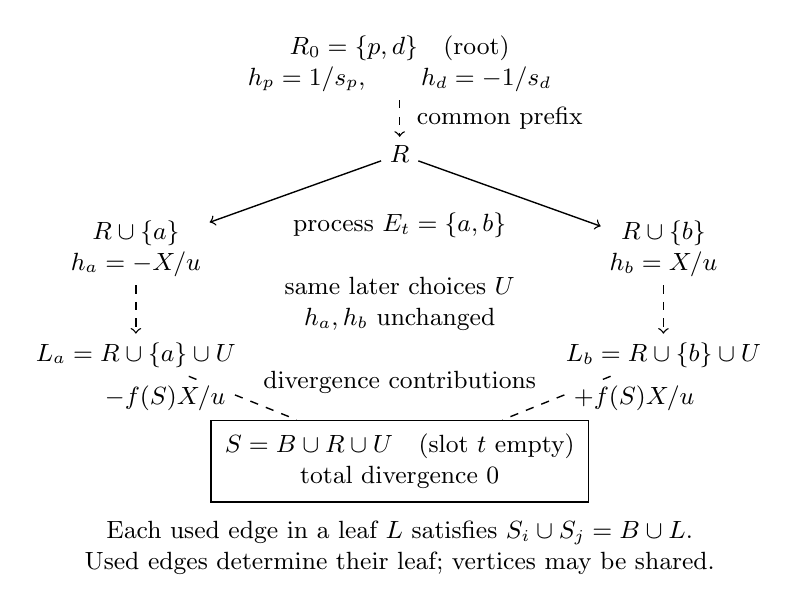
\begin{tikzpicture}[
  x=1cm,y=1cm,
  every node/.style={font=\small,align=center,inner sep=3pt},
  construction/.style={->,line width=0.5pt},
  continuation/.style={->,dashed,line width=0.5pt},
  contribution/.style={dashed,line width=0.5pt}
]
  \node (root) at (0,0)
    {$R_0=\{p,d\}$\quad(root)\\
     $h_p=1/s_p,\qquad h_d=-1/s_d$};
  \node (prefix) at (0,-1.15) {$R$};
  \draw[continuation] (root) -- (prefix)
    node[midway,right=3pt] {common prefix};
  \node at (0,-2.05) {process $E_t=\{a,b\}$};

  \node (childa) at (-3.35,-2.35)
    {$R\cup\{a\}$\\$h_a=-X/u$};
  \node (childb) at (3.35,-2.35)
    {$R\cup\{b\}$\\$h_b=X/u$};
  \draw[construction] (prefix) -- (childa);
  \draw[construction] (prefix) -- (childb);

  \node (leafa) at (-3.35,-3.7) {$L_a=R\cup\{a\}\cup U$};
  \node (leafb) at (3.35,-3.7) {$L_b=R\cup\{b\}\cup U$};
  \draw[continuation] (childa) -- (leafa);
  \draw[continuation] (childb) -- (leafb);
  \node at (0,-3.05) {same later choices $U$\\$h_a,h_b$ unchanged};

  \node[draw,line width=0.5pt,inner sep=5pt] (shared) at (0,-5.05)
    {$S=B\cup R\cup U$\quad(slot $t$ empty)\\
     total divergence $0$};
  \draw[contribution] (leafa) -- (shared)
    node[midway,left=4pt,fill=white,inner sep=2pt] {$-f(S)X/u$};
  \draw[contribution] (leafb) -- (shared)
    node[midway,right=4pt,fill=white,inner sep=2pt] {$+f(S)X/u$};
  \node at (0,-4.05) {divergence contributions};

  \node at (0,-6.15)
    {Each used edge in a leaf $L$ satisfies $S_i\cup S_j=B\cup L$.\\
     Used edges determine their leaf; vertices may be shared.};
\end{tikzpicture}

\caption{The recursive split and cancellation of an ordinary-hole
divergence.  Here $X=\sum_{i\in R}h_i(R)s_i^a$, and $u$ is the common
new-hole total.  Let $U$ contain one selected element from every ordinary
slot processed after $t$.  Using the same $U$ gives the two
leaves $L_a,L_b$ and their shared state $S=B\cup R\cup U$.
Its two divergence contributions cancel.  The lines describe analytical
construction and contributions, not chain transitions or current
directions.  Leaf flows may share vertices but use disjoint edges;
states missing $p$ or $d$ each have one leaf representation.
The algorithm does not compute this recursion.}
\label{fig:transport}
\end{figure}

The resulting flow has the required divergences and energy at most
$\Phi_m$.  Equations \eqref{eq:flowcriterion} and
\eqref{eq:potentialbound} prove \eqref{eq:transport}.
The construction also covers $m=0$, when there is only the root clique.
\end{proof}

\section{A chain and its observable Poincar\'e bound}\label{sec:chain}

We now apply transport to a Metropolis chain on transversals and defect
states.  The target is a variance bound that retains all values on
transversals and only the mean within each defect class.  We prove its
two components separately before combining them.

Fix $q\in(0,1]$.  For each defect type $ij$, choose a positive multiplier
$w_{ij}$, and define
\begin{equation}\label{eq:chainweights}
 \lambda(S)=
 \begin{cases}
 f_q(S),&S\in\Om_0,\\
 w_{ij}f_q(S),&S\in\Om_{ij},
 \end{cases}
 \qquad
 \Lambda=\sum_{S\in\Om}\lambda(S),\qquad \pi(S)=\frac{\lambda(S)}\Lambda.
\end{equation}
The conditional law on transversals is
$\mu(S)=f_q(S)/c_0$ for $S\in\Om_0$; it does not depend on the
multipliers.  Call the multipliers \emph{good} if
\begin{equation}\label{eq:good}
 \frac14w^*_{ij}\le w_{ij}\le4w^*_{ij},
 \qquad w^*_{ij}=\frac{c_0}{c_{ij}}.
\end{equation}
For good multipliers,
\begin{equation}\label{eq:typemasses}
 \Lambda\le5n^2c_0,\qquad
 \pi(\Om_0)\ge\frac1{5n^2},\qquad
 \pi(\Om_{ij})\ge\frac1{20n^2}.
\end{equation}
Indeed each defect has total multiplied weight between $c_0/4$ and
$4c_0$, and there are $n(n-1)$ defects.

\paragraph{The Metropolis chain.}
At a state $S$, stay put with probability $1/2$.  Otherwise choose
uniformly and independently $a\in S$ and $b\in V\setminus S$, and
propose $S'=S\setminus\{a\}\cup\{b\}$.  Reject if $S'\notin\Om$;
otherwise accept with probability $\min\{1,\lambda(S')/\lambda(S)\}$.
Write $P$ for its transition matrix.

This is a reversible chain with stationary law $\pi$.  It is irreducible:
any two transversals are connected by flips within pairs, and each defect
can reach a transversal by moving an element from its full pair to its
empty pair.  All these transitions have positive probability.  It is
lazy, with $P(S,S)\ge1/2$.

For $H:\Om\to\R$, define the unnormalized energy
\begin{equation}\label{eq:D}
 D(H)=\sum_{\substack{\{S,S'\}\\S,S'\in\Om,\ |S\triangle S'|=2}}
   \min\{\lambda(S),\lambda(S')\}\bigl(H(S)-H(S')\bigr)^2.
\end{equation}
Each undirected edge is counted once.  The Dirichlet form is
\begin{equation}\label{eq:Dirichlet}
 \calE(H)=\inner{H}{(I-P)H}_\pi=\frac{D(H)}{2n^2\Lambda}.
\end{equation}
Here $\inner{G}{H}_\pi=\sum_S\pi(S)G(S)H(S)$.

\subsection{Variation on transversals}

The first application recursively conditions the transversal law.
At each node, the defect-total inequalities select a pair for which
the transport coefficient is bounded, and variance decomposition
assembles the resulting estimates.

\begin{lemma}\label{lem:transversalvariance}
For good multipliers and every $H:\Om\to\R$,
\begin{equation}\label{eq:transversalvariance}
 \Var_\mu H\le C_{\rm p}\frac{D(H)}{c_0},
 \qquad C_{\rm p}=n(1+8n).
\end{equation}
\end{lemma}

\begin{proof}
We construct a binary tree that successively conditions the transversal
law.  We choose each branching pair to control the transport coefficient
at that node.  At a node with partial assignment $\sigma$, set
\[
 a_{ij}=\frac{c^{\sigma}_{ij}}{z_{\sigma}}\frac{c_{ji}}{c_0}
 \quad (i\ne j\text{ unassigned}).
\]
\Cref{lem:coefficient}, used both conditionally and with the global
indices reversed, gives
\begin{equation}\label{eq:scores}
 a_{ij}a_{ji}\le\frac1{16},\qquad
 a_{ij}a_{jk}\le a_{ik}\quad(i,j,k\text{ distinct}).
\end{equation}
Draw an arc $i\to j$ when $a_{ij}>1$.  There is no two-cycle, and arcs
are transitive on distinct vertices.  A shortest directed cycle of
length at least three would therefore have a shorter cycle.  The graph
is acyclic and has a sink $k$.  Thus
\begin{equation}\label{eq:sink}
 \frac{c^{\sigma}_{kt}}{z_{\sigma}}\frac{c_{tk}}{c_0}\le1
 \quad\text{for every other unassigned pair }t.
\end{equation}
If only one pair remains, take that pair and the condition is vacuous.
Branch by specifying which element of pair $k$ is chosen.

Apply \Cref{lem:transport} with the assignment $\sigma$ fixed, the two
elements of pair $k$ as singleton slots $p,d$, and the other unassigned
pairs as ordinary slots.  The class $\mathcal X_p$ selects $d$, and
$\mathcal X_d$ selects $p$.  They are the two children, so
$s_p+s_d=z_{\sigma}$ and $W_p=W_d=1$.  If ordinary slot $t$ is empty, pair
$k$ is full; hence $W_t=w_{tk}$.  Also $v_t=c^{\sigma}_{kt}$.  Goodness and
\eqref{eq:sink} imply
\begin{equation}\label{eq:sinkbound}
 \frac{v_t}{W_t}\le4\frac{c^{\sigma}_{kt}c_{tk}}{c_0}\le4z_{\sigma}.
\end{equation}
Let $D_{\sigma}(H)$ be the sum in \eqref{eq:D} over all edges whose endpoints
respect $\sigma$.  The transport graph is a subgraph of this graph with the
same unnormalized conductances.  Multiplying \eqref{eq:transport} by $s_ps_d/z_{\sigma}$
therefore yields
\begin{equation}\label{eq:nodevariance}
 \frac{s_ps_d}{z_{\sigma}}(\overline H_p-\overline H_d)^2
 \le\left(1+\frac2{z_{\sigma}}\sum_t\frac{v_t}{W_t}\right)D_{\sigma}(H)
 \le(1+8n)D_{\sigma}(H).
\end{equation}

Unnormalized variance decomposition at every node says that
$c_0\Var_\mu H$ is the sum of the left side of \eqref{eq:nodevariance}
over all internal nodes; the leaves are singleton transversals.
At any fixed depth, the sets of vertices respecting different nodes are
disjoint.  Indeed, two nodes inherit contradictory choices at the pair
where their paths first diverged, even though later choices of branching
pair may differ.  Hence the sum of $D_{\sigma}(H)$ at that depth is at most
$D(H)$.  There are $n$ internal depths, giving
\eqref{eq:transversalvariance}.
\end{proof}

\subsection{Means of defect classes}

The second application connects a whole defect class to a transversal
event of probability at least one quarter.  The preceding variance
bound then connects that conditional mean to the full transversal mean.

Let $\overline H_T=\E_\pi[H\mid\Om_T]$.  Within each type the multiplier
is constant, so this is also the conditional mean for unmultiplied
weights $f_q$.

\begin{lemma}\label{lem:defecttransfer}
Assume the multipliers are good, and let $H:\Om\to\R$.
For each defect type $ij$ there is an event $\mathcal A\subseteq\Om_0$
obtained by prescribing the selected elements in pairs $i,j$, with
$\mu(\mathcal A)\ge1/4$.  Its conditional mean
$\overline H'=\E_\mu[H\mid\mathcal A]$ satisfies
\begin{equation}\label{eq:defecttransfer}
 (\overline H_{ij}-\overline H')^2
       \le C_{\rm d}\frac{D(H)}{c_0},
 \qquad C_{\rm d}=8+32n,
\end{equation}
and
\begin{equation}\label{eq:conditionalmean}
 (\overline H'-\overline H_0)^2\le4\Var_\mu H.
\end{equation}
\end{lemma}

\begin{proof}
Among the four assignments at pairs $i,j$, choose one whose transversal
total is at least $c_0/4$.  Denote its chosen elements by $a_i,a_j$ and
their mates by $b_i,b_j$, and let $\mathcal A$ be this transversal event.
In \Cref{lem:transport}, set
\[
 B=\{a_j\},\qquad C=\{b_i\},\qquad p=a_i,\qquad d=b_j,
\]
and use the remaining original pairs as ordinary slots.  The singleton
slots now belong to different original pairs.  For any ordinary
slot $E_t=\{x_t,y_t\}$, the following display records the selected
elements in pairs $i,j,t$.  Here $u_t$ is either element of $E_t$,
and every other ordinary pair is singly occupied:
\[
\begin{array}{c|ccc}
 &\text{pair }i&\text{pair }j&\text{pair }t\\ \hline
 \mathcal X_p&\varnothing&\{a_j,b_j\}&\{u_t\}\\
 \mathcal X_d&\{a_i\}&\{a_j\}&\{u_t\}\\
 \mathcal X_t&\{a_i\}&\{a_j,b_j\}&\varnothing\\
 \text{sets counted by }v_t&\varnothing&\{a_j\}&E_t
\end{array}
\]
Thus $\mathcal X_p=\Om_{ij}$ and $\mathcal X_d=\mathcal A$, giving
\[
 s_p=c_{ij},\quad W_p=w_{ij},\quad s_d\ge c_0/4,\quad W_d=1.
\]
For an ordinary hole $t$, the class $\mathcal X_t$ is contained in
$\Om_{tj}$, with the choice $a_i$ fixed at pair $i$, so $W_t=w_{tj}$.
The sets counted by $v_t$ lie outside $\mathcal X$: both singleton
slots are missing and $E_t$ is doubled.  In the original pairing they
form the subset of $\Om_{it}$ with $a_j$ selected, so $v_t\le c_{it}$.

The first two terms of the coefficient in \eqref{eq:transport} are each
at most $4/c_0$.  For each ordinary slot, goodness and
\Cref{lem:coefficient} give
\[
 \frac{2v_t}{s_ps_dW_t}
 \le\frac{8c_{it}c_{tj}}{c_{ij}s_dc_0}
 \le\frac8{s_d}\le\frac{32}{c_0}.
\]
The transport subgraph again uses the unnormalized conductances in $D$, so
\eqref{eq:defecttransfer} follows.  Finally, since $\mu(\mathcal A)\ge1/4$, Jensen's inequality on
$\mathcal A$ gives \eqref{eq:conditionalmean}.
\end{proof}

Define $\Qproj$ on functions on $\Om$ by retaining every value on
$\Om_0$ and replacing the values on each defect class by that class's
conditional mean.  It is the orthogonal projection in $L^2(\pi)$ onto
the functions that are constant on each defect class.  It fixes
constants and preserves expectations.  This is the block-averaging operator
for the partition with one singleton block for each transversal and one
block for each defect class.
The bound below is a partition-restricted Poincar\'e inequality in the
sense of \cite[Definition~4]{CVY2026}.

The inequality below controls $\Qproj H$, not every fluctuation of
$H$ within a defect class.  This is precisely the distinction needed
for the two simulation estimates in \Cref{sec:probability}.

\begin{proposition}[Observable Poincar\'e inequality]\label{prop:observable}
For good multipliers and every $H:\Om\to\R$,
\begin{equation}\label{eq:observable}
 \Var_\pi(\Qproj H)\le K_{\rm obs}\calE(H),
 \qquad K_{\rm obs}=2000n^6.
\end{equation}
\end{proposition}

\begin{proof}
Bound the variance by the squared deviation from $\overline H_0$.
By \Cref{lem:transversalvariance,lem:defecttransfer},
\begin{align*}
 \Var_\pi(\Qproj H)
 &\le \pi(\Om_0)\Var_\mu H
       +\sum_{ij}\pi(\Om_{ij})(\overline H_{ij}-\overline H_0)^2\\
 &\le \Var_\mu H+2C_{\rm d}\frac{D(H)}{c_0}+8\Var_\mu H\\
 &\le (9C_{\rm p}+2C_{\rm d})\frac{D(H)}{c_0}.
\end{align*}
Using \Cref{eq:typemasses,eq:Dirichlet}, the final expression is at most
\[
 10n^4(72n^2+73n+16)\calE(H)
 \le1610n^6\calE(H)<2000n^6\calE(H).
\]
\end{proof}

\section{Two consequences for simulation}\label{sec:probability}

We need two controls of the chain: accurate time averages of observables
fixed by $\Qproj$, and mixing of the trace that records successive visits
to $\Om_0$.  The averages learn type probabilities and annealing ratios;
the trace supplies warm transversal starts for those averages.
The proofs use finite reversible-chain facts about correlated averages,
traces, and return times; see \cite[Sections~2.7.1 and~4.4.1,
Corollary~2.24]{AldousFill2002}.  We include the arguments to retain
their exact normalizations and warm-start hypotheses.

\subsection{Time averages from a warm start}

The stationary estimate is the restricted-Poincar\'e empirical-average
bound of Chen, Vigoda, and Yang
\cite[Theorem~5(ii) and Section~3.6]{CVY2026}.  Its dual-energy argument
also has the earlier antecedent of Kipnis and Varadhan
\cite[Section~3]{KipnisVaradhan1985}.  We include the finite-chain proof
and extend it to a warm start by domination of trajectory laws.

For probability distributions $\nu,\pi$ on a finite set, write
$\nu\le U\pi$ to mean pointwise domination.  Such a start is called
$U$-warm.

\begin{lemma}\label{lem:timeaverages}
Suppose the multipliers are good.  If $G=\Qproj G$ and a trajectory
$(X_t)$ of $P$ starts with law $\nu\le U\pi$, then for every integer
$N\ge1$,
\begin{equation}\label{eq:MSE}
 \E_\nu\left[\left(\frac1N\sum_{t=0}^{N-1}G(X_t)-\E_\pi G\right)^2\right]
 \le\frac{2UK_{\rm obs}\Var_\pi G}{N}.
\end{equation}
\end{lemma}

\begin{proof}
First start in stationarity and put $g=G-\E_\pi G$.  For any $H$,
orthogonality of the projection and \eqref{eq:observable} imply
\[
 |\inner{g}{H}_\pi|^2
 =|\inner{g}{\Qproj H}_\pi|^2
 \le\Var_\pi G\,\Var_\pi(\Qproj H)
 \le K_{\rm obs}\Var_\pi G\,\calE(H).
\]
On the mean-zero subspace $I-P$ is invertible, because $P$ is finite and
irreducible.  Take $H=(I-P)^{-1}g$ and use
$\calE(H)=\inner{g}{H}_\pi$.  This gives
\begin{equation}\label{eq:resolvent}
 \inner{g}{(I-P)^{-1}g}_\pi\le K_{\rm obs}\Var_\pi G.
\end{equation}
Reversibility makes $P$ self-adjoint, and laziness puts its eigenvalues
on the mean-zero subspace in $[0,1)$.  Indeed $P=(I+R)/2$ for a
reversible stochastic matrix $R$, whose spectrum lies in $[-1,1]$.
Consequently,
\[
 \inner{g}{(I-P)^{-1}g}_\pi
   =\sum_{t\ge0}\inner{g}{P^tg}_\pi,
 \qquad \inner{g}{P^tg}_\pi\ge0.
\]
In the variance of the stationary average, the coefficient of each of
these covariances is at most $2/N$.  This proves \eqref{eq:MSE} for
$U=1$.  Finally, $\nu\le U\pi$ implies the same domination for the
entire trajectory law.  Applying it to the nonnegative squared error
proves the general case.
\end{proof}

\subsection{The trace on transversals}

Set $A=\Om_0$.  Starting from $x\in A$, let
$\tau_A^+=\min\{t\ge1:X_t\in A\}$.  The \emph{trace transition}
$P_A(x,y)=\Prob_x(X_{\tau_A^+}=y)$ records the next visit to $A$, including
a possible visit at time one.  All hitting and return times have finite
expectation, since the underlying chain is finite and irreducible.
For completeness, from every state there is a positive-probability path
to $A$ of bounded length; taking the minimum of these finitely many
positive path probabilities gives a geometric tail in blocks of that
length.

\begin{lemma}\label{lem:trace}
With good multipliers, $P_A$ is reversible with stationary law $\mu$,
irreducible, and lazy.  Its inverse spectral gap is at most $18n^4$.
In particular, for every integer $s\ge0$,
\begin{equation}\label{eq:tracemixing}
 \left|\frac{P_A^s(x,y)}{\mu(y)}-1\right|
 \le\frac{\exp(-s/(18n^4))}{\min_{z\in A}\mu(z)}
 \quad(x,y\in A).
\end{equation}
If a trace step begins with a law $\nu\le U\mu$, its expected number of
underlying transitions is at most
\begin{equation}\label{eq:returncost}
 \frac{U}{\pi(A)}\le5Un^2.
\end{equation}
\end{lemma}

\begin{proof}
For $h:A\to\R$, let $H$ be its harmonic extension: $H=h$ on $A$ and
$H(x)=\E_x[h(X_{\tau_A})]$ off $A$, where
$\tau_A=\min\{t\ge0:X_t\in A\}$.  Conditioning on the first step gives
\[
 (I-P)H=0\ \text{ off }A,\qquad
 ((I-P)H)|_A=(I-P_A)h.
\]
For two such extensions, symmetry of $I-P$ implies symmetry of
$I-P_A$ in $L^2(\mu)$, since $\pi|_A=\pi(A)\mu$.  Thus $P_A$ is
reversible and $\mu$ is stationary.  Irreducibility follows by tracing
paths in the original chain, and $P_A(x,x)\ge P(x,x)\ge1/2$.
Taking the same extension in both slots gives
\begin{equation}\label{eq:traceenergy}
 \calE(H)=\pi(A)\inner{h}{(I-P_A)h}_\mu.
\end{equation}
Because $\pi(A)=c_0/\Lambda$, \eqref{eq:Dirichlet} gives
$D(H)/c_0=2n^2\calE(H)/\pi(A)$.  Applying
\Cref{lem:transversalvariance} to $H$ therefore yields
\[
 \Var_\mu h\le2n^2C_{\rm p}\inner{h}{(I-P_A)h}_\mu,
 \qquad 2n^2C_{\rm p}\le18n^4.
\]
This proves the spectral-gap bound.  Laziness makes every nonconstant
trace eigenvalue nonnegative.  Applying the centered operator norm
bound to the point densities at $x,y$, whose centered $L^2(\mu)$ norms
are at most $\mu(x)^{-1/2},\mu(y)^{-1/2}$, gives
\[
 \left|\frac{P_A^s(x,y)}{\mu(y)}-1\right|
 \le\frac{(1-1/(18n^4))^s}{\sqrt{\mu(x)\mu(y)}},
\]
which implies \eqref{eq:tracemixing}.

To prove the cost statement, start a return excursion with distribution
$\mu$ and let $v(z)$ be the expected number of visits to $z$ at times
$0,\ldots,\tau_A^+-1$.  Multiplying $v$ by $P$ shifts these expected
occupations to times $1,\ldots,\tau_A^+$.  The initial and final laws
are both $\mu$, so $vP=v$.  By uniqueness of the stationary law, $v$ is
a scalar multiple of $\pi$.  Since $v|_A=\mu$, that scalar is
$1/\pi(A)$.  Summing over $z$ proves
$\E_\mu\tau_A^+=1/\pi(A)$.  Domination of the starting law gives the
factor $U$, and \eqref{eq:typemasses} finishes \eqref{eq:returncost}.
\end{proof}

\section{Annealing and learning the multipliers}\label{sec:algorithm}

The initial transversal weight is known at $q=1$.  We estimate its
successive ratios as $q$ decreases, while learning multipliers that
keep every type sufficiently frequent.  The trace supplies a fresh
warm start for each estimation phase, and the observable variance
bound controls the resulting averages.
The frequency-ratio updates and balancing of defect totals adapt the
interpolation strategy of Jerrum, Sinclair, and Vigoda \cite{JSV2004};
the warm restarts below use the trace and observable estimates proved here.

We first specify a run with constant success probability using exact
rational random choices.  The next section gives a bounded-bit
implementation and amplification.  The feasibility test in
\Cref{sec:reduction} is performed before these runs.

\subsection{Parameters and the schedule}

Let $b$ be the least nonnegative integer with $2^{-b}\le\epsilon/10$,
and set
\begin{equation}\label{eq:schedule}
 \rho=1-\frac1{2n},\qquad L=2n(n+b),\qquad
 q_j=\rho^j\ (0\le j\le L),\qquad
 \eta=\frac{\epsilon}{32(L+1)}.
\end{equation}
The restart and estimation routines use three integer parameters:
\begin{equation}\label{eq:parameters}
 \begin{split}
 \tau&=20n^4\bigl(n(L+1)+2\bigr),\\
 B_{\rm restart}&=2000(L+1)^2n^2\tau,\\
 N_{\rm av}&=\left\lceil\frac{10^{10}(L+1)n^{14}}{\eta^2}\right\rceil.
 \end{split}
\end{equation}
Here $\tau$ is the number of trace transitions at each restart stage,
$B_{\rm restart}$ caps the total underlying transition attempts in one
restart, and $N_{\rm av}$ is the number of observations in one estimation
phase.  We make no attempt to optimize these polynomial bounds.

Bernoulli's inequality and $1-x\le e^{-x}$ give
\begin{equation}\label{eq:schedulebounds}
 \rho^n\ge\frac12,\qquad
 \rho^{2n}\le e^{-1}<\frac12,\qquad
 2^{-L}\le q_L\le2^{-(n+b)}.
\end{equation}
For every state and every $j<L$,
\begin{equation}\label{eq:stepweight}
 \frac12\le\frac{f_{q_{j+1}}(S)}{f_{q_j}(S)}
       =\rho^{d(S)}\le1.
\end{equation}
The same inequalities hold for each ratio $c_T(q_{j+1})/c_T(q_j)$.
Thus the ideal multiplier $w^*_{ij}=c_0/c_{ij}$ changes by a factor
between $1/2$ and $2$ per phase.  Write $\mu_j$ for the transversal law
at $q_j$.  Equation \eqref{eq:stepweight} also gives
\begin{equation}\label{eq:mudrift}
 \mu_j\le2\mu_{j+1}.
\end{equation}

\subsection{One run}

At $q_0=1$, $\mu_0$ is uniform on the $2^n$ transversals, $c_0=2^n$,
and $c_{ij}=2^{n-2}$ whenever a defect type exists.  Initialize
$w^{(0)}_{ij}=4$.  Store every subsequent phase's multipliers as they
are learned.

The observations used to learn these multipliers also reveal the
preceding trajectory's endpoint.  After conditioning on that history,
the endpoint need not satisfy the polynomial warm-start bound needed
below.  Each phase therefore generates a fresh starting transversal
from the known law $\mu_0$, through the stored parameter levels and with
independent randomness.

For $j=0,\ldots,L-1$, perform the following steps.  Any abort mentioned
below returns zero from the run.

\begin{enumerate}[label=\textbf{\arabic*.},leftmargin=*]
\item \textbf{Restart to obtain a warm transversal.}
Start from a uniform transversal, using $n$ fair bits.  For
$a=1,\ldots,j$, perform $\tau$ trace transitions at parameter $q_a$
with the stored multipliers $w^{(a)}$.  Each trace transition is
implemented by running the underlying Metropolis chain until the next
visit to $\Om_0$, at a strictly positive time.  The endpoint of one
stage is the starting transversal of the next.  Before attempting an
underlying transition, reserve one unit from a budget of
$B_{\rm restart}$ for this entire restart; if no unit remains, abort
before drawing any bits for that transition.
For $j=0$, simply use the initial uniform transversal.  All randomness
for this restart is independent of the previous phase history.

\item \textbf{Estimate type probabilities and a ratio.}
Using fresh random bits, run the chain from that transversal at
$q_j,w^{(j)}$ and observe
$N_{\rm av}$ consecutive states, including the starting state.  Let
$\widehat p_T$ be the empirical average of $\one_{\Om_T}$ for every
type $T\in\mathcal T$, and let $\widehat u$ be the empirical average of
\begin{equation}\label{eq:ratioobservable}
 G_j(S)=\one_{\Om_0}(S)\rho^{d(S)}.
\end{equation}
Abort if any $\widehat p_T$ is zero.

\item \textbf{Record the ratio and update the multipliers.}
Set
\begin{equation}\label{eq:updates}
 \widehat R_j=\frac{\widehat u}{\widehat p_0}.
\end{equation}
If $j+1<L$, set, for every defect type,
\begin{equation}\label{eq:weightupdate}
 w^{(j+1)}_{ij}=w^{(j)}_{ij}\frac{\widehat p_0}{\widehat p_{ij}}.
\end{equation}
This estimates the current ideal multiplier; the superscript $j+1$
records the phase in which it will be used.  The factor-two drift in
the ideal multiplier permits using an accurate estimate at the next
parameter while retaining the factor-four bound in \eqref{eq:good}.
\end{enumerate}
If every phase completes, output
\begin{equation}\label{eq:estimator}
 \widehat Z=2^n\prod_{j=0}^{L-1}\widehat R_j.
\end{equation}

\subsection{Warm restarts and estimation error}

Condition on any complete previous phase history in which all stored
multipliers are good at their respective parameters.  Under this
conditioning the fresh restart uses fixed kernels and independent
randomness, starting from the known law $\mu_0$.  Analyze the uncapped
restart and its subsequent observations; the capped process agrees
whenever the restart finishes within its cap.

Uniformly over all phases and all transversals, \eqref{eq:schedulebounds}
gives
\begin{equation}\label{eq:minmu}
 \mu_j(S)\ge\frac{q_L^n}{2^n}\ge2^{-n(L+1)}.
\end{equation}
By \Cref{lem:trace} and \eqref{eq:parameters}, after $\tau$ trace
transitions the density relative to the current $\mu_a$ lies between
$1/2$ and $3/2$, from any initial distribution.  Indeed,
\[
 \exp\bigl(-\tau/(18n^4)\bigr)\,2^{n(L+1)}\le\tfrac12.
\]
At the start of each stage the law is at most $4\mu_a$: at the previous
parameter it is at most twice that parameter's transversal law, and
\eqref{eq:mudrift} costs at most a further factor of two.  For the
first stage the starting law is exactly $\mu_0$.  Pointwise domination
by $4\mu_a$ persists through the stage because $\mu_a$ is stationary
for its trace.  Thus \eqref{eq:returncost}, applied at each trace step,
implies
\begin{equation}\label{eq:restartmean}
 \E[\text{underlying transitions in the restart}]
 \le20n^2L\tau.
\end{equation}
Markov's inequality yields
\begin{equation}\label{eq:restartfailure}
 \Prob[\text{restart exceeds }B_{\rm restart}]
 \le\frac{L}{100(L+1)^2}\le\frac1{32(L+1)}.
\end{equation}

The endpoint law of the uncapped restart is at most $2\mu_j$,
including the case $j=0$.  Since $\pi(\Om_0)\ge1/(5n^2)$, it is at
most $10n^2\pi$, where $\pi$ is the enlarged chain's stationary law at
the current parameters.  Every type indicator and $G_j$ belongs to the
range of $\Qproj$ and takes values in $[0,1]$.  Their stationary means
are
\begin{equation}\label{eq:stationarymeans}
 p_T=\pi(\Om_T),\qquad
 u=p_0R_j,\qquad R_j=\frac{c_0(q_{j+1})}{c_0(q_j)}.
\end{equation}
All these means are at least $1/(20n^2)$, by
\Cref{eq:typemasses,eq:stepweight}.
\Cref{lem:timeaverages} bounds the mean squared error of each empirical
average around its stationary mean by
\begin{equation}\label{eq:averageMSE}
 \frac{40000n^8}{N_{\rm av}}.
\end{equation}
There are $n(n-1)+2\le2n^2$ observables.  Applying Markov's inequality
to each squared error and taking a union bound gives
\begin{align}
 \Prob\bigl[\text{some relative error exceeds }\eta\bigr]
 &\le 2n^2\frac{40000n^8}{N_{\rm av}}
                       \frac{400n^4}{\eta^2}\notag\\
 &\le\frac{0.0032}{L+1}\le\frac1{32(L+1)}.
 \label{eq:estimationfailure}
\end{align}
Both error probabilities were bounded in the uncapped experiment.
Their union contains failure of the actual phase, since the two
simulations agree whenever the restart finishes within its cap.
When neither event occurs, all empirical type probabilities are positive
and no zero-count abort occurs.

\subsection{Induction on learned weights}

On a phase with all relative errors at most $\eta$, the exact identity
\[
 w^{(j)}_{ij}\frac{p_0}{p_{ij}}=\frac{c_0(q_j)}{c_{ij}(q_j)}
\]
shows that \eqref{eq:weightupdate} estimates the current ideal multiplier
within factors $(1-\eta)/(1+\eta)$ and its reciprocal.  These factors
lie between $1/2$ and $2$.  The ideal multiplier changes by at most a
factor of two at the next parameter, so the new multipliers are good
for phase $j+1$.

Initialization is ideal.  Conditional on any previously successful
history, \Cref{eq:restartfailure,eq:estimationfailure} bound the next
phase's failure probability by $1/[16(L+1)]$.  Induction and a union
bound over all $L$ phases therefore give
\begin{equation}\label{eq:analyticfailure}
 \Prob[\text{some restart abort or inaccurate phase}]\le\frac1{16}.
\end{equation}
\subsection{Accuracy of the product}

On the complementary event in \eqref{eq:analyticfailure},
\begin{equation}\label{eq:ratioerror}
 \frac{1-\eta}{1+\eta}\le\frac{\widehat R_j}{R_j}
               \le\frac{1+\eta}{1-\eta}.
\end{equation}
Since $\eta<1/2$ and
$\log((1+\eta)/(1-\eta))\le4\eta$, the telescoping product satisfies
\[
 e^{-4L\eta}\le\frac{\widehat Z}{c_0(q_L)}\le e^{4L\eta}.
\]
Here $c_0(q_0)=2^n$.  Equation \eqref{eq:schedule} gives
$4L\eta\le\epsilon/8$, and for $0<\epsilon<1$,
\begin{equation}\label{eq:productaccuracy}
 (1-\epsilon/4)c_0(q_L)\le\widehat Z
                         \le(1+\epsilon/4)c_0(q_L).
\end{equation}
Every transversal basis of $K$ has weight one; every other transversal
has weight at most $q_L$.  Therefore, writing $Z=Z(M_1,M_2)$,
\begin{equation}\label{eq:contamination}
 Z\le c_0(q_L)\le Z+2^nq_L
       \le Z+\epsilon/10\le(1+\epsilon/10)Z,
\end{equation}
where the final inequality uses the feasibility test, $Z\ge1$.
Combining \Cref{eq:productaccuracy,eq:contamination} gives
\[
 (1-\epsilon)Z\le\widehat Z\le(1+\epsilon)Z.
\]
Thus the run using exact random choices has success probability at
least $15/16$.

\section{Oracle implementation, bit bounds, and amplification}
\label{sec:implementation}

We now implement the run with independent fair bits and bound all work
on every execution, including those with inaccurate estimates or aborts.

\subsection{States and oracle weights}

Represent a state by its $2n$-bit indicator.  Its occupancy pattern, a
proposed exchange, and membership in $\Om$ can be computed in polynomial
time.  For $S\subseteq V$, let $S_x,S_y\subseteq[n]$ be its positions
in the two copies.  The required rank is
\begin{equation}\label{eq:oracleweight}
 \rank_K(S)=\rank_{M_1}(S_x)+|S_y|-r
                              +\rank_{M_2}([n]\setminus S_y).
\end{equation}
Both original ranks are computed greedily.  This takes at most $2n$
original independence queries, with polynomial overhead for constructing
their $n$-bit indicators.  Consequently no oracle other than the two
given independence oracles is needed.

\subsection{Sizes of the rational numbers}

The integer $b$ in \eqref{eq:schedule} is $O(\ell)$ and can be found
using shifts and binary comparisons.  Thus $L$ is polynomial in
$n,\ell$.  The integers $\tau,B_{\rm restart},N_{\rm av}$ are polynomial
in $n,\ell,\epsilon^{-1}$, since
$\eta^{-1}=32(L+1)\epsilon^{-1}$.

We may store unreduced numerator--denominator pairs throughout.  If
$C_T$ is a type count among the $N_{\rm av}$ observations, then the
multiplier update is multiplication by $C_0/C_{ij}$.  A zero denominator
causes an abort before division.  After at most $L$ phases, all
multiplier numerators and denominators have bit length
\begin{equation}\label{eq:multiplierbits}
 O\bigl(1+L\log(N_{\rm av}+1)\bigr).
\end{equation}
This bound holds even when the empirical estimates are inaccurate.

For $0\le d\le n$, the observable $\rho^d$ has common denominator
$(2n)^n$ and integer numerator $(2n-1)^d(2n)^{n-d}$.  If $X_t$ denotes
the $t$th observation in phase $j$ and $C_0>0$ counts the transversals
among those observations,
the exact implementation is
\begin{equation}\label{eq:integeraccumulator}
 A_j=\sum_{\substack{0\le t<N_{\rm av}\\X_t\in\Om_0}}
       (2n-1)^{d(X_t)}(2n)^{n-d(X_t)},
 \qquad \widehat R_j=\frac{A_j}{(2n)^nC_0}.
\end{equation}
The accumulator has bit length
$O(\log(N_{\rm av}+1)+n\log(2n))$.  The rational product
\eqref{eq:estimator} has bit length
\begin{equation}\label{eq:outputbits}
 O\bigl(n+L\log(N_{\rm av}+1)+Ln\log(2n)\bigr).
\end{equation}

Finally, $q_j^d=((2n-1)/(2n))^{jd}$ has numerator and denominator bit
length $O(1+Ln\log(2n))$.  Together with
\eqref{eq:multiplierbits}, this bounds the sizes of state weights,
acceptance fractions, and all comparisons by a fixed polynomial.
Each state weight is formed directly from its rank deficiency, the
stored multiplier of its type, and $q_j^{d(S)}$.
Integer arithmetic on these lengths, including multiplication,
division, and comparison, takes polynomial bit operations.

\subsection{Exact rational choices with bounded trials}

To draw uniformly from $\{0,\ldots,v-1\}$, use
$\lceil\log_2v\rceil$ unbiased bits and reject values at least $v$.
For $v=1$, return zero without drawing bits.  With unrestricted trials
the distribution is exactly uniform, and every trial succeeds with
probability at least $1/2$.  A rational acceptance probability $a/v$
is implemented by checking whether this uniform integer is less than
$a$.  The denominators have polynomial bit length by the preceding
subsection.

With the restart attempt caps, a run uses at most
\begin{equation}\label{eq:drawcount}
 M=3L(B_{\rm restart}+N_{\rm av})
\end{equation}
uniform-integer calls: two for the proposed exchange and one for its
acceptance, per underlying transition.  Laziness and initial uniform
transversals use fair bits directly.  Choose the least positive integer
$D_{\rm bits}$ satisfying
\begin{equation}\label{eq:bitcap}
 M2^{-D_{\rm bits}}\le1/32.
\end{equation}
Allow at most $D_{\rm bits}$ trials in each uniform-integer call; if all
fail, abort the run and return zero.  The cap is
$O(1+\log M)$.  Couple this procedure with the unrestricted-trial one
using the same random bits up to an abort.  Conditional on the previous
history, a call exceeds its cap with probability at most
$2^{-D_{\rm bits}}$, even if its denominator depends on that history.
A union bound over \eqref{eq:drawcount} therefore bounds the coupling
failure probability by $1/32$.

Combining this with \eqref{eq:analyticfailure}, the bounded run succeeds
with probability at least
\begin{equation}\label{eq:runsuccess}
 1-\frac1{16}-\frac1{32}=\frac{29}{32}>\frac34.
\end{equation}
Every execution has at most $L(B_{\rm restart}+N_{\rm av})$ underlying
transition attempts, including any attempt interrupted by a bit-cap
abort.  If $h_{\max}$ is the polynomial bound on the bit lengths of
uniform-integer denominators established above, the total number of
random bits is at most
\[
 nL+L(B_{\rm restart}+N_{\rm av})+MD_{\rm bits}h_{\max}.
\]
The first two terms cover initial transversals and laziness.  Together
with \eqref{eq:oracleweight} and the rational size bounds, this proves
polynomial oracle and bit-operation bounds for a run.  In particular,
exceptional histories affect success probability but cannot cause an
unbounded execution.

\subsection{Amplification and completion of the proof}

Let $b_\delta$ be the least nonnegative integer with
$2^{-b_\delta}\le\delta$, and perform
$J=10b_\delta+1$ independent bounded runs after the feasibility pretest.
Return their rational median.  The number $J$ is odd and is
$O(1+\log\delta^{-1})$.

For each run let $X$ be its failure indicator relative to the desired
interval $[(1-\epsilon)Z,(1+\epsilon)Z]$.  By
\eqref{eq:runsuccess}, $\E[2^X]\le5/4$.  Independence and Markov's
inequality imply
\[
 \Prob[\text{at least half the runs fail}]
 \le\left(\frac{5}{4\sqrt2}\right)^J
 \le2^{-b_\delta}\le\delta,
\]
using $(5/(4\sqrt2))^{10}<1/2$.  If a strict majority of estimates lie
in the desired interval, so does their median.  Computing $b_\delta$
and comparing rational estimates costs polynomial bit operations,
including the dependence on $\ell$.

For an infeasible input the deterministic pretest returns zero.  If
$n=0$, the unique common basis is empty and the initial output is one.
For all remaining ranks, including $r=0$ and $r=n$, the preceding
argument applies.  Every output is a nonnegative rational, and all
complexity bounds are uniform over the two promised independence
oracles.  This proves \Cref{thm:main}.

\section{Counting and sampling common independent sets}
\label{sec:intersection}

The equal-rank common-bases theorem also gives counting and sampling
algorithms for common independent sets when the input ranks differ.
Truncation reduces prescribed-cardinality counting to common bases;
self-reduction then supplies sampling.

\begin{corollary}[Common independent sets]\label{cor:intersection}
Let $M_1,M_2$ be arbitrary matroids on an explicitly enumerated ground
set $[n]$, supplied by fixed exact independence oracles with $n$-bit
subset queries.  Their ranks may differ.  For an integer $k$, let
$\mathcal C_k$ consist of the $k$-element subsets of $[n]$ independent
in both matroids, and put
\[
 \mathcal C=\bigcup_{j=0}^n\mathcal C_j,\qquad
 h=\max_{I\in\mathcal C}|I|,\qquad
 \mathcal C_{\max}=\mathcal C_h.
\]
The maximum $h$ is well defined because $\varnothing\in\mathcal C$.
Each family $\mathcal F\in\{\mathcal C_k,\mathcal C,\mathcal C_{\max}\}$
has the following algorithms.
\begin{enumerate}[label=(\roman*)]
\item Given rational $\epsilon,\delta\in(0,1)$, a randomized oracle
algorithm returns a nonnegative rational $\widehat N$ satisfying
\[
 \Prob\bigl[(1-\epsilon)|\mathcal F|\le\widehat N
                         \le(1+\epsilon)|\mathcal F|\bigr]\ge1-\delta.
\]
If $\mathcal F=\varnothing$, an exact pretest returns $0$ before
randomization.  On every execution, oracle calls and other bit operations
are bounded by a fixed polynomial in
$n,\ell,\epsilon^{-1},\log\delta^{-1}$.
\item Given rational $\theta\in(0,1)$, a randomized oracle algorithm
decides emptiness exactly.  If $\mathcal F=\varnothing$, it returns a
distinguished symbol $\bot$.  Otherwise it returns $S\in\mathcal F$ on
every execution, and its output law satisfies
\[
 d_{\rm TV}\bigl(\mathcal L(S),\operatorname{Unif}(\mathcal F)\bigr)
 =\frac12\sum_{I\in\mathcal F}
       \left|\Prob[S=I]-\frac1{|\mathcal F|}\right|\le\theta.
\]
On every execution, oracle calls and other bit operations are bounded by
a fixed polynomial in $n,\ell,\theta^{-1}$.
\end{enumerate}
Here $\ell$ is the binary encoding length of the numerical inputs to the
algorithm in question, including $k$ only for $\mathcal C_k$.
Both algorithms use only the two given independence oracles and
independent unbiased random bits.
\end{corollary}

The counting-to-generation principle for self-reducible families is
classical \cite[Section~6]{JVV1986}.  The direct argument below records
the exact independence-oracle interface, the total-variation error, and
the work bound on every execution.

\begin{proof}[Proof of Corollary~\ref{cor:intersection}]
\textbf{Counting by truncation.}
Use the deterministic matroid-intersection algorithm
\cite[Section~41.2, Theorem~41.4]{Schrijver2003}, already invoked in
\Cref{sec:reduction}, to find the maximum common independent-set size
$h$.  Its input permits different ranks and requires only the promised
matroid axioms, a common explicit ground set, and exact independence
oracles.  If $k<0$ or $k>h$, then $\mathcal C_k$ is empty, so return
$0$ for its count.  If $k=0$, return $1$.  For $0<k\le h$, define the
truncation $T_k(M_i)$ by declaring $J$ independent exactly when it is
independent in $M_i$ and $|J|\le k$.  Both truncations have rank exactly
$k$: a common independent set of size $h$ contains an independent
$k$-set in each matroid.  Their common bases are therefore precisely
$\mathcal C_k$.  A truncation query uses at most one original
independence query and a cardinality check, so \Cref{thm:main} applies
with the required oracle and bit bounds even if the original ranks
differ.

For $\mathcal C$, estimate each $|\mathcal C_j|$, $0\le j\le h$, with
relative error $\epsilon$ and failure probability $\delta/(h+1)$, and
add the nonnegative rational estimates.  With probability at least
$1-\delta$, all estimates satisfy their relative bounds
simultaneously.  Adding those bounds gives
\[
 (1-\epsilon)|\mathcal C|
 \le\sum_{j=0}^h\widehat N_j
 \le(1+\epsilon)|\mathcal C|.
\]
There are at most $n+1$ terms.  For $\mathcal C_{\max}$, use the
prescribed-cardinality procedure at $k=h$.  The families $\mathcal C$
and $\mathcal C_{\max}$ are always nonempty; when $h=0$, both consist
only of the empty set.  The feasibility tests thus handle every
zero-count case exactly.  Since
$\log((h+1)/\delta)=O(\log(n+1)+\log\delta^{-1})$, the confidence
allocation preserves the stated fully polynomial counting bound.

\textbf{Exact feasibility during self-reduction.}
For sampling, first perform the same exact emptiness test, returning
$\bot$ if the requested family is empty.  If $n=0$, return
$\varnothing$.  Otherwise initialize $A=D=\varnothing$.  Maintain
disjoint sets $A,D$ of included and excluded elements, with $A$ common
independent and at least one requested set consistent with these choices, and let
$R=[n]\setminus(A\cup D)$ be the remaining ground set.  Define $N_i$
on $R$ by declaring, for $J\subseteq R$,
\begin{equation}\label{eq:intersectionminor}
 J\text{ independent in }N_i
 \quad\Longleftrightarrow\quad
 A\cup J\text{ independent in }M_i.
\end{equation}
The empty set is independent because $A$ is, and heredity and
augmentation follow from those of $M_i$.  Thus $N_i$ is a matroid,
namely the restriction to $R$ of the contraction $M_i/A$.
After relabeling $R$, an exact query to either residual minor uses
one original query and polynomial work to construct its $n$-bit
indicator.

If $R=\varnothing$, return $A$.  Otherwise let $e$ be the least element
of $R$.  The exclusion branch has included
set $A$ and excluded set $D\cup\{e\}$.  Before constructing the
inclusion branch, test whether
$A\cup\{e\}$ is independent in both original matroids; if not, that
branch is empty.  Otherwise that branch has included set $A\cup\{e\}$
and excluded set $D$, and
\eqref{eq:intersectionminor} again supplies valid minor oracles.
The remaining ground set in either branch is $R\setminus\{e\}$.
For a prescribed original cardinality $t$, including the case $t=h$
for maximum-cardinality sampling, the branch with decision
$b\in\{0,1\}$ has as many completions as the residual pair has common
independent sets of size $t-|A|-b$.  The prescribed-cardinality
pretest above decides exactly whether this count is zero; the original
target $t$ stays fixed throughout the recursion.  For
unrestricted cardinality, the branch count is the all-cardinalities
count of the residual pair; it is positive whenever the branch's
included set is common independent.  These descriptions partition the
current feasible completions into two smaller instances, at least one
of which is nonempty.

\textbf{Branch probabilities and sampling error.}
Let $a_0,a_1$ be their true counts.  For comparison, the ideal
recursion with access to these counts chooses the inclusion branch with probability
$p=a_1/(a_0+a_1)$; induction on $|R|$ shows that it is uniform on the
requested family.  The actual recursion follows the unique feasible
branch deterministically when only one exists.  When both are feasible,
obtain fresh estimates $\widehat a_0,\widehat a_1$ from the appropriate
counter, each with relative tolerance and failure probability
\[
 \alpha=\frac{\theta}{4n},\qquad
 \beta=\frac{\theta}{8n}.
\]
If $\widehat a_0+\widehat a_1=0$, set $\widehat p=0$; this selects a
known-feasible branch.  Otherwise set
$\widehat p=\widehat a_1/(\widehat a_0+\widehat a_1)$.
This rule does not mistake a zero estimate on an inaccurate run for
proof that a branch is empty.

Let $s$ be the least nonnegative integer with
$2^{-s}\le\theta/(4n)$, and put
\[
 p_s=2^{-s}\lfloor 2^s\widehat p\rfloor.
\]
Use exactly $s$ fresh unbiased bits to obtain a uniform integer in
$\{0,\ldots,2^s-1\}$ and choose inclusion when it is less than
$2^sp_s$.  This implements $p_s$ with
$|p_s-\widehat p|<2^{-s}$, without an unbounded rejection procedure.

When both estimates are accurate, write
$\widehat a_b=a_b(1+u_b)$ with $|u_b|\le\alpha$.  Since $a_0,a_1>0$,
\[
 |\widehat p-p|
 =\frac{a_0a_1|u_1-u_0|}
 {(a_0+a_1)\bigl(a_0(1+u_0)+a_1(1+u_1)\bigr)}
 \le\frac{\alpha}{2(1-\alpha)}
 \le\alpha,
\]
where the last inequality uses $\alpha<1/2$.  Conditional on every
shared history of the ideal and actual recursions, fresh randomness
makes the probability that either estimate is inaccurate at most $2\beta$.
Couple their next decisions; the conditional probability that they
separate is at most
\[
 \alpha+2\beta+2^{-s}\le\frac{3\theta}{4n}.
\]
This also holds at a forced decision, where the probability is zero.
A sequential coupling over at most $n$ decisions now gives
\[
 d_{\rm TV}\bigl(\mathcal L(S),\operatorname{Unif}(\mathcal F)\bigr)
 \le n\bigl(\alpha+2\beta+2^{-s}\bigr)
 \le\frac{3\theta}{4}<\theta.
\]
The exact branch tests keep every output in the requested family, including on
executions with inaccurate estimates.

Finally, each sampling step uses at most two counter calls and
polynomial exact matroid-intersection work.  An all-cardinalities
counter uses at most $n+1$ common-bases calls.  The derived parameters
satisfy $\alpha^{-1}=4n/\theta$,
$\log\beta^{-1}=O(1+\log n+\log\theta^{-1})$, and
$s=O(1+\log n+\log\theta^{-1})$.  Their binary encodings have polynomial
length, and $s$ can be found by shifts and rational comparisons.
The every-execution bound in \Cref{thm:main} bounds the lengths
of the returned rationals; summing at most $n+1$ such rationals,
forming $\widehat p$, and computing its dyadic rounding therefore take
polynomial bit operations.  Together with
\eqref{eq:intersectionminor}, these observations give the asserted
oracle and bit bounds on every execution.
\end{proof}

\clearpage

\begin{thebibliography}{CFJMYZ25}

\bibitem[AF02]{AldousFill2002}
David Aldous and James Allen Fill.
\newblock {\em Reversible Markov Chains and Random Walks on Graphs}.
\newblock Unfinished monograph, 2002, recompiled 2014.
\newblock \url{https://www.stat.berkeley.edu/~aldous/RWG/book.html}.

\bibitem[AASV23]{AASV2021}
Yeganeh Alimohammadi, Nima Anari, Kirankumar Shiragur, and Thuy-Duong Vuong.
\newblock Fractionally log-concave and sector-stable polynomials:
  Counting planar matchings and more.
\newblock arXiv:2102.02708, version~3, April 3, 2023; first posted 2021.
\newblock \url{https://arxiv.org/abs/2102.02708v3}.

\bibitem[ALOV24]{ALOV2024}
Nima Anari, Kuikui Liu, Shayan {Oveis Gharan}, and Cynthia Vinzant.
\newblock Log-concave polynomials {II}: High-dimensional walks and an {FPRAS}
  for counting bases of a matroid.
\newblock {\em Annals of Mathematics}, 199(1):259--299, 2024.
\newblock \url{https://doi.org/10.4007/annals.2024.199.1.4}.
\newblock Preprint locators refer to arXiv version~3, January 18, 2019:
  \url{https://arxiv.org/abs/1811.01816v3}.

\bibitem[AO17]{AO2017}
Nima Anari and Shayan {Oveis Gharan}.
\newblock A generalization of permanent inequalities and applications
  in counting and optimization.
\newblock arXiv:1702.02937, version~1, February 9, 2017.
\newblock \url{https://arxiv.org/abs/1702.02937v1}.

\bibitem[AOR16]{AOR2016}
Nima Anari, Shayan {Oveis Gharan}, and Alireza Rezaei.
\newblock Monte Carlo Markov chain algorithms for sampling strongly
  Rayleigh distributions and determinantal point processes.
\newblock In {\em 29th Annual Conference on Learning Theory},
  volume~49 of {\em Proceedings of Machine Learning Research},
  pages 103--115. PMLR, 2016.
\newblock \url{https://proceedings.mlr.press/v49/anari16.html}.

\bibitem[AOV21]{AOV2021}
Nima Anari, Shayan {Oveis Gharan}, and Cynthia Vinzant.
\newblock Log-concave polynomials, {I}: Entropy and a deterministic
  approximation algorithm for counting bases of matroids.
\newblock {\em Duke Mathematical Journal}, 170(16):3459--3504, 2021.
\newblock \url{https://doi.org/10.1215/00127094-2020-0091}.
\newblock Preprint locators refer to arXiv version~2, November 5, 2018:
  \url{https://arxiv.org/abs/1807.00929v2}.

\bibitem[BS07]{BS2007}
Alexander Barvinok and Alex Samorodnitsky.
\newblock Random weighting, asymptotic counting, and inverse isoperimetry.
\newblock {\em Israel Journal of Mathematics}, 158:159--191, 2007.
\newblock \url{https://doi.org/10.1007/s11856-007-0008-8}.
\newblock Preprint version~2, June 4, 2003:
  \url{https://arxiv.org/abs/math/0302177v2}.

\bibitem[BH19]{BrandenHuh2018}
Petter Br{\"a}nd{\'e}n and June Huh.
\newblock Hodge--Riemann relations for Potts model partition functions.
\newblock arXiv:1811.01696, version~2, February 11, 2019; first posted 2018.
\newblock \url{https://arxiv.org/abs/1811.01696v2}.

\bibitem[BH20]{BH2020}
Petter Br{\"a}nd{\'e}n and June Huh.
\newblock Lorentzian polynomials.
\newblock {\em Annals of Mathematics}, 192(3):821--891, 2020.
\newblock \url{https://doi.org/10.4007/annals.2020.192.3.4}.

\bibitem[CFJMYZ25]{CFJMYZ2025}
Xiaoyu Chen, Weiming Feng, Zhe Ju, Tianshun Miao, Yitong Yin, and Xinyuan Zhang.
\newblock Faster mixing of the Jerrum--Sinclair chain.
\newblock arXiv:2504.02740, version~1, April 3, 2025.
\newblock \url{https://arxiv.org/abs/2504.02740v1}.

\bibitem[CVY26]{CVY2026}
Xiaoyu Chen, Eric Vigoda, and Xiongxin Yang.
\newblock Faster {FPRAS} for the permanent via restricted {Poincar\'e}
  inequalities and coupled flows.
\newblock arXiv:2608.26599, version~1, August 27, 2026.
\newblock \url{https://arxiv.org/abs/2608.26599v1}.

\bibitem[CGM21]{CGM2021}
Mary Cryan, Heng Guo, and Giorgos Mousa.
\newblock Modified log-Sobolev inequalities for strongly log-concave
  distributions.
\newblock {\em Annals of Probability}, 49(1):506--525, 2021.
\newblock \url{https://doi.org/10.1214/20-AOP1453}.
\newblock Preprint locators refer to arXiv version~4, August 8, 2020:
  \url{https://arxiv.org/abs/1903.06081v4}.

\bibitem[DS06]{DoyleSnell2006}
Peter G. Doyle and J. Laurie Snell.
\newblock {\em Random Walks and Electric Networks}.
\newblock Web edition dated July 5, 2006, derived from the 1984 MAA book.
\newblock \url{https://math.dartmouth.edu/~doyle/docs/walkspdf/walks.pdf}.

\bibitem[Edm79]{Edmonds1979}
Jack Edmonds.
\newblock Matroid intersection.
\newblock In {\em Discrete Optimization {I}}, volume~4 of {\em Annals of
  Discrete Mathematics}, pages 39--49. North-Holland, 1979.
\newblock \url{https://doi.org/10.1016/S0167-5060(08)70817-3}.

\bibitem[FM92]{FM1992}
Tom{\'a}s Feder and Milena Mihail.
\newblock Balanced matroids.
\newblock In {\em Proceedings of the Twenty-Fourth Annual ACM Symposium
  on Theory of Computing}, pages 26--38. Association for Computing
  Machinery, 1992.
\newblock \url{https://doi.org/10.1145/129712.129716}.

\bibitem[JSV04]{JSV2004}
Mark Jerrum, Alistair Sinclair, and Eric Vigoda.
\newblock A polynomial-time approximation algorithm for the permanent of a
  matrix with nonnegative entries.
\newblock {\em Journal of the ACM}, 51(4):671--697, 2004.
\newblock \url{https://doi.org/10.1145/1008731.1008738}.

\bibitem[JVV86]{JVV1986}
Mark R. Jerrum, Leslie G. Valiant, and Vijay V. Vazirani.
\newblock Random generation of combinatorial structures from a uniform
  distribution.
\newblock {\em Theoretical Computer Science}, 43(2--3):169--188, 1986.
\newblock \url{https://doi.org/10.1016/0304-3975(86)90174-X}.

\bibitem[KV85]{KipnisVaradhan1985}
Claude Kipnis and S. R. S. Varadhan.
\newblock Central limit theorems for additive functionals of reversible
  Markov chains and applications.
\newblock {\em Ast{\'e}risque}, 132:65--70, 1985.
\newblock \url{https://www.numdam.org/item/AST_1985__132__65_0/}.

\bibitem[Liu23]{Liu2023}
Kuikui Liu.
\newblock {\em Spectral Independence: A New Tool to Analyze {Markov} Chains}.
\newblock PhD thesis, University of Washington, 2023.
\newblock Section 13.2, Problem 1, p. 197.
  \url{https://kuikuiliu.github.io/files/dissertation.pdf}.

\bibitem[Sch03]{Schrijver2003}
Alexander Schrijver.
\newblock {\em Combinatorial Optimization: Polyhedra and Efficiency}, volume~24
  of {\em Algorithms and Combinatorics}.
\newblock Springer, Berlin, 2003.
\newblock \url{https://homepages.cwi.nl/~lex/co/}.

\bibitem[SV16]{SV2016}
Damian Straszak and Nisheeth K. Vishnoi.
\newblock Real stable polynomials and matroids: Optimization and counting.
\newblock arXiv:1611.04548, version~1, November 14, 2016.
\newblock \url{https://arxiv.org/abs/1611.04548v1}.

\end{thebibliography}

\end{document}
